% Adapted from J. Leon, https://tex.stackexchange.com/questions/432312/how-do-i-draw-an-lstm-cell-in-tikz
\usetikzlibrary{positioning, fit, arrows.meta, shapes, calc}

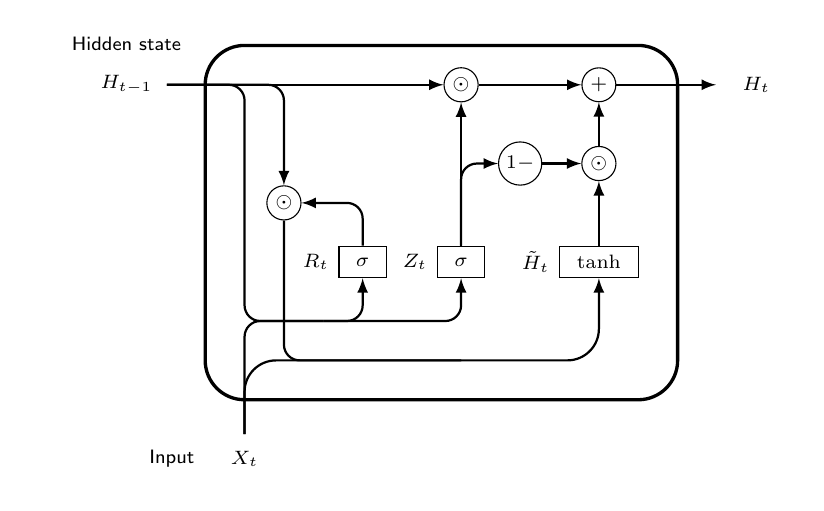
\begin{tikzpicture}[
    font=\sf \scriptsize,
    >=latex,
    % Styles
    cell/.style={
        rectangle,
        rounded corners=5mm,
        draw,
        very thick,
        },
    operator/.style={
        circle,
        draw,
        inner sep=1.5pt,
        minimum height =0.4cm,
        },
    function/.style={
        ellipse,
        draw,
        inner sep=2pt
        },
    ct/.style={
        line width = .75pt,
        minimum height=0.60cm,
        minimum width=1cm,
        inner sep=2pt,
        },
    gt/.style={
        rectangle,
        draw,
        minimum width=0.6cm,
        minimum height=0.4cm,
        inner sep=2pt
        },
    inoutlabels/.style={
        text width=2cm,
        align=center,
        },
    Arrow/.style={
        rounded corners=.2cm,
        thick,
        },
    Arrow2/.style={
        rounded corners=.4cm,
        thick,
        },
    ]

    \node [cell, minimum height =4.5cm, minimum width=6cm] at (0,0){} ;

    \node [gt, label={left:$\boldsymbol{R}_{t}$}] (ibox1) at (-1,-0.5) {$\sigma$};
    \node [gt, label={left:$\boldsymbol{Z}_{t}$}] (ibox2) at (0.25,-0.5) {$\sigma$};
    \node [gt, minimum width=1cm, label={left:$\boldsymbol{\tilde{H}}_{t}$}] (ibox3) at (2,-0.5) {$\tanh$};

    \node [operator] (mux1) at (-2,0.25) {$\odot$};
    \node [operator] (mux2) at (0.25,1.75) {$\odot$};
    \node [operator] (add1) at (2,1.75) {$+$};
    \node [operator] (sub) at (1,0.75) {$1-$};
    \node [operator] (mux3) at (2,0.75) {$\odot$};

    \node[ct, label={[inoutlabels]Hidden state}] (h) at (-4,1.75) {$\boldsymbol{H}_{t-1}$};
    \node[ct, label={[inoutlabels, align=right]left:Input}] (x) at (-2.5,-3) {$\boldsymbol{X}_{t}$};

    \coordinate (inputibox1) at ($ (mux1) + (-0.5,0) $);
    \coordinate (inputibox2) at ($ (ibox1) + (-0.5,-0.75) $);
    \coordinate (midbottom) at ($ (ibox2) + (0,-1.25) $);

    \node[ct] (h2) at (4,1.75) {$\boldsymbol{H}_{t}$};

    %\draw [Arrow] (c) -- (mux1) -- (add1) -- (c2);
    \draw [->, Arrow] (h) -| (mux1);
    \draw [->, Arrow] (h) -- (mux2);
    \draw [->, Arrow] (ibox1) |- (mux1);
    \draw [->, Arrow] (ibox2) -- (mux2);
    \draw [->, Arrow] (ibox2) |- (sub);
    \draw [->, Arrow] (sub) -- (mux3);
    \draw [->, Arrow] (ibox3) -- (mux3);
    \draw [->, Arrow] (mux3) -- (add1);
    \draw [->, Arrow] (mux2) -- (add1);
    \draw [->, Arrow] (add1) -- (h2);

    \draw [-, Arrow] (h) -| (inputibox1) |- (inputibox2);
    \draw [->, Arrow] (inputibox2) -| (ibox1);
    \draw [->, Arrow] (inputibox2) -| (ibox2);
    \draw [-, Arrow] (mux1) |- (midbottom);
    \draw [->, Arrow2] (midbottom) -| (ibox3);
    \draw [-, Arrow2] (x) |- (midbottom);
    \draw [-, Arrow] (x) |- (inputibox2);
\end{tikzpicture}
